\documentclass[twocolumn]{article}

\usepackage{scrextend}
\changefontsizes{8pt}

\makeatletter
\renewcommand*{\fps@figure}{!htb}
\renewcommand*{\fps@table}{!htb}
\makeatother

\usepackage{sectsty}
\sectionfont{\fontsize{11}{11}\selectfont}
\subsectionfont{\fontsize{10}{11}\selectfont}

% \usepackage[compact]{titlesec}
% \titlespacing{\section}{0pt}{2ex}{1ex}
% \titlespacing{\subsection}{0pt}{1ex}{1ex}
% \titlespacing{\subsubsection}{0pt}{0.5ex}{1ex}

\setlength{\parskip}{0cm}
\setlength{\parindent}{1em}

\usepackage{geometry}
 \geometry{
 a4paper,
 total={170mm,257mm},
 left=20mm,
 top=20mm,
 }
\usepackage[utf8]{inputenc}
\usepackage[hidelinks]{hyperref}
\usepackage{amsmath, bm}
\usepackage[ruled,vlined]{algorithm2e}
\usepackage{amssymb}
\usepackage{graphicx}
\usepackage{float}
\usepackage{booktabs}
\usepackage[parfill]{parskip}
\usepackage{comment}
\usepackage{subcaption}
\usepackage{booktabs}



\usepackage{listings}
\lstset{
    language=Python,
    breaklines=true,
    breakatwhitespace=true,
    basicstyle=\footnotesize,
    frame=lines
}
\usepackage[capitalise, nameinlink]{cleveref}

\usepackage[sorting=none, style=verbose]{biblatex}
\addbibresource{lab_4.bib}

\usepackage{titling}
\setlength{\droptitle}{-1cm}

\title{\Large COMP6248 Lab 3 Exercise -- Optimise it!}
\author{\small Wei Chien Teoh (Eugene)\\\bigskip \href{mailto:wct1c16@soton.ac.uk}{wct1c16@soton.ac.uk}}
\date{\small 29 April 2021}

\begin{document}

\maketitle

\section*{Introduction}

The results are seeded using \lstinline{torch.manual_seed(0)} to provide reproducible results.

\section{Wide MLPs on MNIST}

\subsection{Wider MLPs}

\cref{fig:learning-curves} illustrates the learning curve for different width of the MLP. It can be observed that the validation curve starts to diverge from the minima with around 5000 neurons in the hidden layer. The divergence increases as the hidden size increases after that point.

By intuition, deep networks are better at generalising because it is able to learn features with increasing level of abstractions \autocite{eldanPowerDepthFeedforward2016}. Shallow and wide networks tend to memorise the structure of the features, thus causing them to have bad generalisation.

As the width of the MLP increases, the model complexity increases, which allows the model to approximate functions of higher order. This is useful to learning the structure of the dataset. However, increasing model complexity comes with the cause of learning the structure of that particular dataset, hence will be unable to have good performance when unseen data of similar structure is given.



\begin{figure}
    \centering
    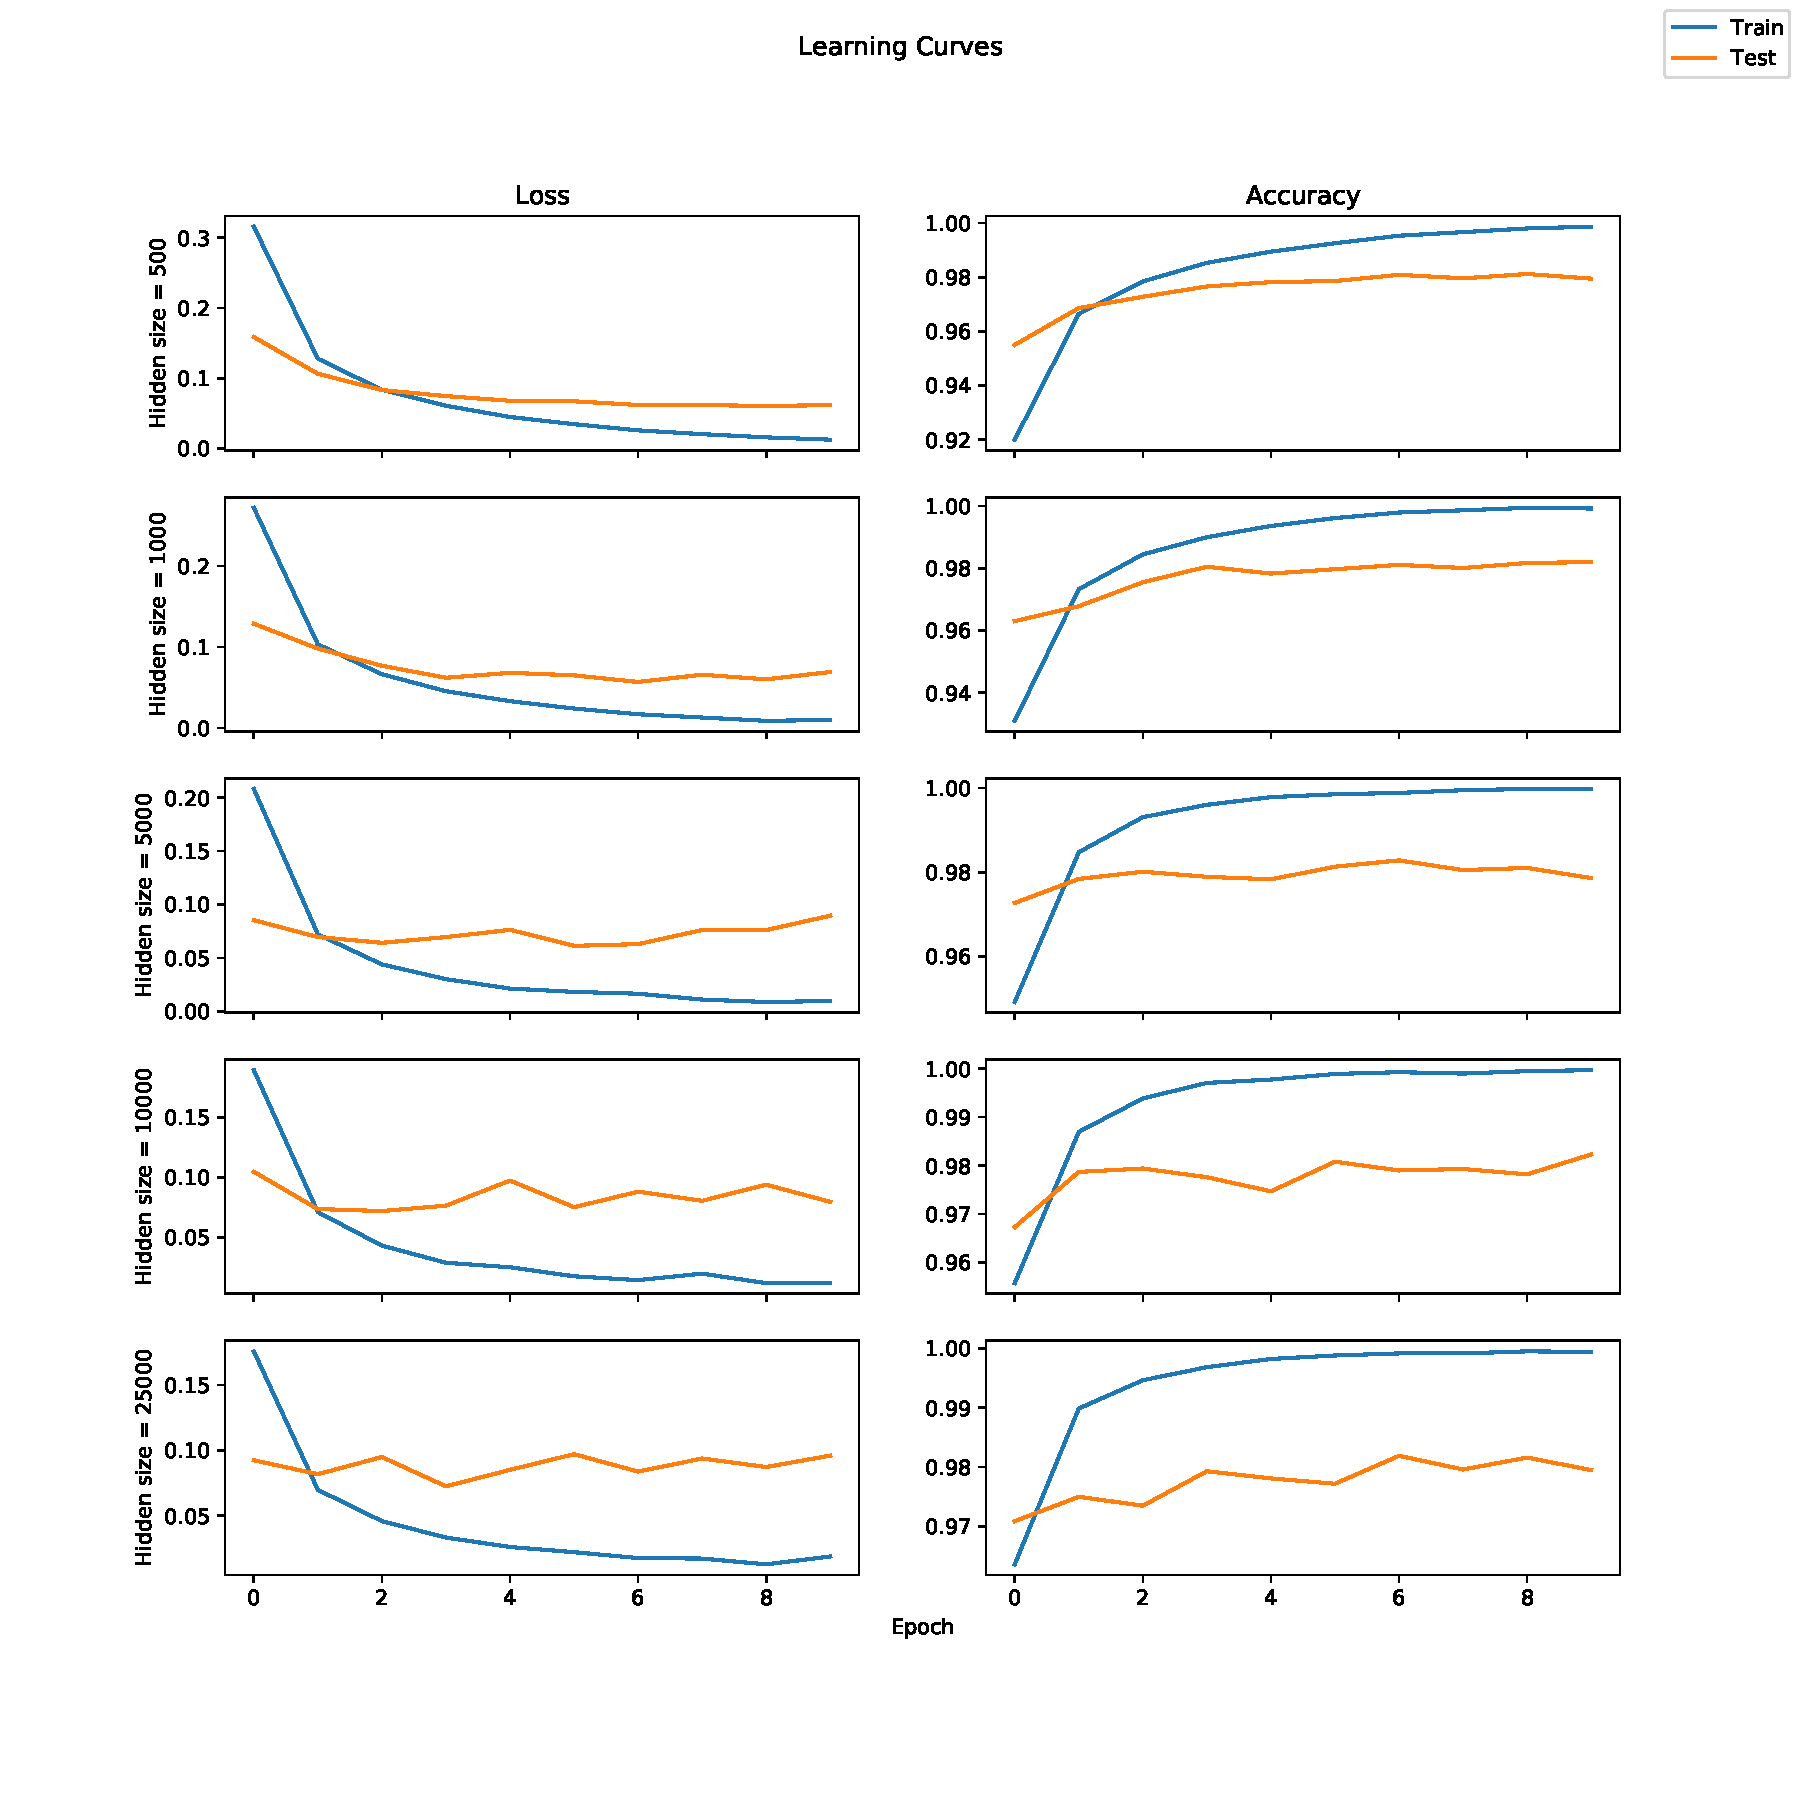
\includegraphics[width=\linewidth]{Figures/learning_curves.pdf}
    \caption{Learning curves for different number of hidden layer neurons. (Left) Loss Plots. (Right) Accuracy Plots.}
    \label{fig:learning-curves}
\end{figure}

\end{document}